\PassOptionsToPackage{unicode,pdfusetitle}{hyperref}
\PassOptionsToPackage{hyphens}{url}
\PassOptionsToPackage{dvipsnames,svgnames,x11names}{xcolor}

\documentclass[10pt]{beamer}

\usetheme{moloch}
\usefonttheme{professionalfonts}
\setbeamertemplate{page number in head/foot}[appendixframenumber]

\usepackage[T1]{fontenc}
\usepackage{lmodern}
\usepackage{bm}
\usepackage{amssymb,amsmath,mathtools,amsthm}
\usepackage{textcomp}
\usepackage{pifont}
\usepackage{dirtree}
\usepackage{siunitx}

\usepackage{upquote} % straight quotes in verbatim environments
\usepackage{microtype}
\UseMicrotypeSet[protrusion]{basicmath} % disable protrusion for tt fonts

\usepackage{xmpmulti}

% listings
\usepackage{listings}

% Define a custom color
\definecolor{backcolour}{rgb}{0.95,0.95,0.95}
\definecolor{codegreen}{rgb}{0,0.6,0}
\definecolor{mygray}{rgb}{0.6,0.6,0.6}

\lstdefinestyle{myStyle}{
  backgroundcolor=\color{backcolour},
  frame=single,
  % commentstyle=\color{codegreen},
  basicstyle=\ttfamily, breakatwhitespace=false, breaklines=true, keepspaces=true,
  numbers=left,
  % numbersep=5pt,
  numberstyle=\footnotesize\color{mygray}, showspaces=false, showstringspaces=false,
  showtabs=false, tabsize=2, }

% Use \lstset to make myStyle the global default
\lstset{style=myStyle}

\usepackage{xcolor}
\usepackage{xurl} % add URL line breaks if available
\usepackage{bookmark}

\usepackage[noabbrev,nameinlink]{cleveref}

\usepackage{hyperref}

\hypersetup{%
  colorlinks = true,
  linkcolor  = mLightGreen,
  filecolor  = mLightGreen,
  citecolor  = mLightGreen,
  urlcolor   = mLightGreen
}

% subfigures
\usepackage{subcaption}

% algorithms
\usepackage[ruled,vlined]{algorithm2e}
\resetcounteronoverlays{algocf}

% tikz and pgfplots stuff
\usepackage{tikz}
\usetikzlibrary{arrows,shapes,positioning,intersections}
\usepackage{pgfplots}
\usepgfplotslibrary{external,colormaps}
\pgfplotsset{compat=1.15}
%\tikzexternalize

% \definecolor{graphicbackground}{rgb}{0.96,0.96,0.8}
% \setbeamercolor{background canvas}{bg=graphicbackground}

\usepackage{booktabs}

% title block
\titlegraphic{\hfill
\includegraphics[height=2.2cm]{images/ucph-vertical.pdf}\vfil}

\title{Normalization and Binary Features}
\subtitle{Intro Presentation}
\author{Johan Larsson}
\institute{Department of Mathemathical Sciences, University of Copenhagen}

% bibliography
\usepackage[style=authoryear,url=false,backend=biber]{biblatex}
\addbibresource{bibliography.bib}


% operators
\DeclareMathOperator*{\argmax}{arg\,max}
\DeclareMathOperator*{\argmin}{arg\,min}
\DeclareMathOperator{\E}{\text{E}}
\DeclareMathOperator{\var}{var}
\DeclareMathOperator{\cov}{cov}
\DeclareMathOperator{\sign}{sign}
\DeclareMathOperator{\card}{card}
\DeclareMathOperator{\cumsum}{cumsum}
\DeclareMathOperator*{\prox}{prox}

% macros
\newcommand{\pkg}[1]{\textsf{#1}}
\renewcommand{\vec}{\vectorsym}
\newcommand{\mat}{\matrixsym}
\newcommand{\du}{\mathrm{d}}

\makeatletter
\newcommand\notsotiny{\@setfontsize\notsotiny\@vipt\@viipt}
\makeatother



\begin{document}

\maketitle

% \begin{frame}[c]
%   \frametitle{Overview}
%
%   \tableofcontents
% \end{frame}

\begin{frame}[c]
  \frametitle{Motivation}

  \begin{itemize}[<+->]
    \item Most regularized methods are scale-sensitive, so have to normalize.
    \item Straightforward normalization when everything is normal, but what about features that have
          other distributions (binary features)?
    \item No literature on the effects of different normalization strategies
  \end{itemize}
\end{frame}

\begin{frame}[c]
  \frametitle{The Elastic Net}

  % Linear regression plus a combination of the \(\ell_1\) and \(\ell_2\) penalties:
  % \begin{equation*}
  %   (\hat{\beta}_0, \hat{\vec{\beta}}) = \argmin_{\beta_0 \in \mathbb{R},\beta \in \mathbb{R}^p} \left( \frac{1}{2} \lVert \vec y - \beta_0 - \mat{X}\vec{\beta} \rVert^2_2  + \lambda_1 \lVert \vec\beta \rVert_1 + \frac{\lambda_2}{2}\lVert \vec \beta \rVert_2^2\right).
  % \end{equation*}
  \begin{equation*}
    \vec{\beta}^* = \operatorname*{minimize}_{\beta \in \mathbb{R}^p} \bigg( \frac{1}{2} \lVert \vec y - \mat{X}\vec{\beta} \rVert^2_2  + \underbrace{\lambda_1 \lVert \vec\beta \rVert_1}_\text{lasso} + \underbrace{\frac{\lambda_2}{2}\lVert \vec \beta \rVert_2^2}_\text{ridge}\bigg)
  \end{equation*}

  \pause

  \begin{figure}
    \centering
    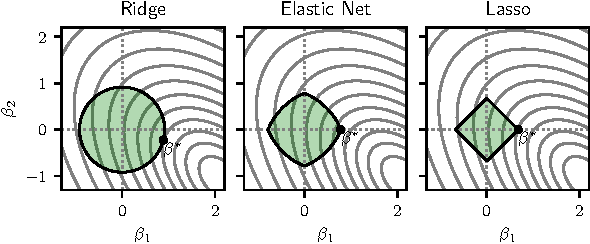
\includegraphics[width=0.85\textwidth]{images/paper6-elasticnet-balls.pdf}
    \caption{%
      The elastic net penalty is a combination of the lasso and ridge penalties. Here shown as a constrained problem.
    }
  \end{figure}
\end{frame}

\begin{frame}[c]
  \frametitle{Sensitivity to Scale}

  Lasso and ridge penalties are \textbf{norms}---feature scales matter!

  \pause

  \begin{exampleblock}{Example}
    Assume
    \[
      \mat{X} \sim \operatorname{Normal}\left(\begin{bmatrix}0 \\ 0\end{bmatrix}, \begin{bmatrix} 4 & 0 \\ 0 & 1\end{bmatrix}\right), \qquad \vec{\beta}^* = \begin{bmatrix} \frac{1}{2} \\ 1 \end{bmatrix}.
    \]

    \medskip\pause

    \begin{table}
      \begin{tabular}{lcc}
        \toprule
        Model & \(\hat{\vec{\beta}}\)                                  & \(\hat{\vec{\beta}}_\text{std}\)                             \\
        \midrule
        OLS   & \(\begin{bmatrix} 0.50 & 1.00\end{bmatrix}^\intercal\) & \(\begin{bmatrix}1.00 & 1.00\end{bmatrix}^\intercal\) \pause \\
        Lasso & \(\begin{bmatrix} 0.38 & 0.50\end{bmatrix}^\intercal\) & \(\begin{bmatrix}0.74 & 0.50\end{bmatrix}^\intercal\) \pause \\
        Ridge & \(\begin{bmatrix} 0.37 & 0.41\end{bmatrix}^\intercal\) & \(\begin{bmatrix}0.74 & 0.41\end{bmatrix}^\intercal\)        \\
        \bottomrule
      \end{tabular}
    \end{table}
  \end{exampleblock}

  \pause

  \alert{Large} scale means \alert{less} penalization because the size of \(\beta_j\) can be smaller for an equivalent effect (on \(\vec{y}\)).

\end{frame}

\begin{frame}[c]
  \frametitle{Normalization}

  \begin{itemize}[<+->]
    \item Scale sensitivity can be mitigated by normalizing the features.
    \item Let \(\tilde{\mat X}\) be the normalized feature matrix, with elements
          \[
            \tilde{x}_{ij} = \frac{x_{ij} - c_{j}}{s_j}.
          \]
    \item After fitting, we transform the coefficients back to their original scale via
          \[
            \hat\beta_j = \frac{\hat\beta^{(n)}_j}{s_j} \quad\text{for}\quad j = 1,2,\dots,p.
          \]
  \end{itemize}

  % \bigskip\pause
  % \begin{block}{Ambiguous Nomenclature}
  %   \begin{itemize}
  %     \item Some refer to this as \emph{standardization} (which we dedicate for the mean--standard deviation combo).
  %     \item Some take normalization to mean \alert{sample-wise} normalization.
  %     \item Some take normalization to mean scaling with a \alert{norm}.
  %     \item Some refer to this (centering and scaling) as \alert{scaling}.
  %   \end{itemize}
  % \end{block}
\end{frame}

\begin{frame}[c]
  \frametitle{Type of Normalization Matters}

  \begin{figure}[htpb]
    \centering
    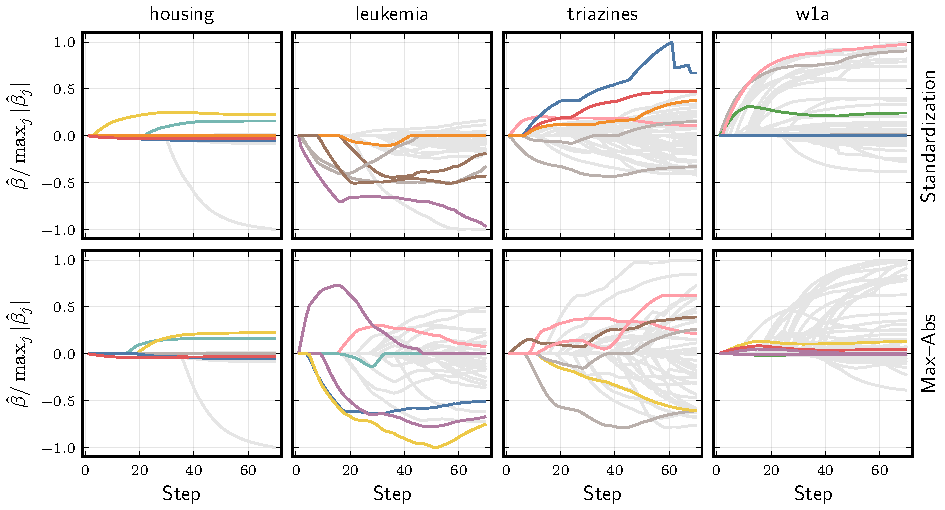
\includegraphics[width=\textwidth]{images/paper6-realdata_paths.pdf}
    \caption{%
      Lasso paths under two different types of normalization (standardization and max--abs normalization). The union of the first five features selected in any of the schemes are colored.
    }
  \end{figure}

\end{frame}

\begin{frame}[c]
  \frametitle{Binary Features}

  \begin{columns}
    \begin{column}{0.45\textwidth}

      For binary features (values 0 and 1 only), we have for the noiseless case
      \[
        \hat{\beta}_j =
        % \frac{\operatorname{S}_{\lambda_1}(\tilde{\vec{x}}^\intercal \vec{y})}{s_j\left(\tilde{\vec{x}}_j^\intercal \tilde{\vec{x}}_j + \lambda_2\right)}
        % =
        \frac{\operatorname{S}_{\lambda_1}\left(\frac{\beta_j^* n \alert{(q - q^2)}}{s_j}\right)}{s_j\left(\frac{n\alert{(q - q^2)}}{s_j^2} + \lambda_2\right)}.
      \]
    \end{column}
    \begin{column}{0.45\textwidth}
      \begin{figure}[htpb]
        \centering
        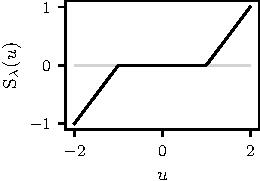
\includegraphics[]{images/paper6-st.pdf}
        \caption{%
          Soft-thresholding
        }
      \end{figure}
    \end{column}
  \end{columns}

  \pause

  \begin{block}{Conclusions}
    \begin{itemize}[<+->]
      \item The elastic net estimator depends on class balance (\(q\)).
      \item \(s_j = q - q^2\) for lasso and \(s_j = \sqrt{q-q^2}\) for ridge removes effect of \(q\).
      \item Suggests the parametrization
            \[
              s_j = (q - q^2)^\delta, \qquad \delta \geq 0.
            \]
    \end{itemize}
  \end{block}

\end{frame}

\begin{frame}[c]
  \frametitle{Mixed Data}

  \begin{figure}[htpb]
    \centering
    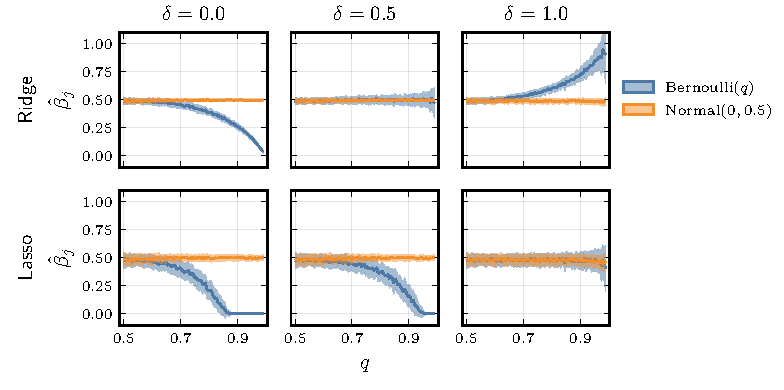
\includegraphics[width=\textwidth]{images/paper6-mixed_data.pdf}
    \caption{%
      Comparison between lasso and ridge estimators for a data set with one binary and one quasi-normal feature.}
  \end{figure}
\end{frame}

\begin{frame}[c]
  \frametitle{Summary}
  \begin{exampleblock}{Contributions}
    \begin{itemize}
      \item As far as we know the first paper to investigate the interplay between normalization and
            regularization
      \item New scaling approach to deal with class-imbalanced binary features
      \item Discussion and suggestions for dealing with mixed data
    \end{itemize}
  \end{exampleblock}

  \pause

  \begin{alertblock}{Limitations}
    \begin{itemize}
      \item So far only theoretical results for limited cases:
            \begin{itemize}
              \item Fixed data (\(\mat{X}\)), normal noise
              \item Orthogonal features
              \item Normal and binary features
            \end{itemize}
    \end{itemize}
  \end{alertblock}
\end{frame}

\begin{frame}[standout]
  Thank you!
\end{frame}

% \begin{frame}[standout]
%   Thank you!
% \end{frame}

% \appendix
% 
% \begin{frame}[allowframebreaks]{References}
%   \printbibliography[heading=none]
% \end{frame}

\end{document}

